
\chapter{Schlussfolgerungen}

Nach der Evaluation und zum Abschluss dieser Arbeit befasst sich dieser Abschnitt mit den gewonnenen Erkenntnissen und zu guter Letzt mit einem Ausblick. 

%\begin{itemize}
%    \item Was sind gute Schlüsselwörte? Sinnvoll im Kontext als Dokumentenbeschrieb oder zusätzliche Informationen?
    %\item Agile und Dokumentation hauptsächlich in Literatur
    %\item TOKEN R/W
%\end{itemize}

%\section{Erkenntnisse} % theoretisch, terminolgoie

%\begin{itemize}
%    \item Sachartikel liefern bessere Resultate als Berichte über Bands
%\end{itemize}

\section{Lessons learned} % Rückmeldungen zum Prozess
Der Projektverlauf war rückblickend erfolgreich: Es ist ein Prototyp entstanden, welcher eine Volltextsuche und eine automatische Extraktion von \gls{Keyphrase}[s] anbietet. 

Dank des agilen Projektmanagements und den wöchentlichen Sitzungen mit dem Projektparter konnte stets auf die neusten Erkenntnisse aus dem Projekt eingegangen werden. Somit war stets gewährleistet, dass das Projekt bestmöglich den Anforderungen des Projektpartners entspricht. Neue Lösungsansätze konnte so innerhalb eines Sprints schnell überprüft werden. Der Umgang mit jeglichen Risiken verlieft problemlos, da der Projektpartner sehr nahe am Entwicklungsprozess eingebunden war. Risiken und Unklarheiten konnten so in einem frühen Stadium erkannt und behandelt werden.

Eine Herausforderung war sicherlich die Abschätzung des Zeithorizonts von den insgesamt 720 Stunden. Durch die wöchentlichen Sitzungen kamen stets viele neue Ideen, Chancen und Verbesserungspotential zum Vorschein. Gleichzeitig sind aber immer die definierten Ziele und Anforderungen präsent. Das Finden einer adäquaten Balance zwischen den fixierten Resultaten und den vielversprechenden neuen Anregungen war nicht immer einfach.

Diese Bachelor-Arbeit bewegt sich sowohl im Feld eines Software- als auch eines Forschungsprojekts. Dadurch waren interessante Einblicke in beide Bereiche möglich. Das agile Projektmanagement war ideal für diese Art von Projekt. Nur so war es möglich, dass die Implementation den ständig wandelnden Ansprüche der Forschung folgen konnte.


%Forschung vs Softwareprojekt Forschung anstelle Software-Projekt

% npm, beta module, modul anpassen für den zweck


\section{Ausblick}

Der Ausblick stellt offene Fragen und zeigt das Potential für die Weiterentwicklung auf. 

\begin{itemize}
    \item Ein nächster, äusserst interessanter Schritt ist eine quantitative Analyse, also ein Vergleich von verschiedenen Algorithmen anhand von Demo-Daten. Dies ist anhand des erarbeiteten Prototypen problemlos möglich. Der Algorithmus verwendet einen festgelegten Schwellenwert zur Bestimmung der wichtigsten extrahierten \gls{Keyphrase}[s]. Ein idealer Wert dafür ist schwierig zu ermitteln. Denn der jetzige Algorithmus liefert je nach Textlänge und Textart sehr unterschiedliche Resultate. Es gilt einen Weg zu finden, welcher unter jeglichen Voraussetzungen sinnvolle Resultate liefert. Dabei ist eine bestimmte Generalität, Abstraktion und Relevanz der Begriffe sehr wichtig. Wie im Stand der Technik beschrieben, existieren noch weitere Algorithmen, welche sich ebenfalls mit ähnlichen Problemstellungen befassen. Sie sind eine Grundlage für weitere Analysen.
    \item Während der Entwicklung stand ein Korpus von etwa 120'000 Dateien zur Verfügung. Grundsätzlich wäre es interessant, verschiedene Korpusgrössen miteinander zu vergleichen. Ab welcher Grösse liefert der Algorithmus überhaupt brauchbare Resultate? Ab wann hat die Grösse keinen Einfluss mehr. Oder ganz generell, was ändert sich an den \gls{Keyphrase}[s] bei einem aktualsierten Korpus? Eventuell macht es gar Sinn den Prototypen direkt mit einem Referenzkorpus auszuliefern. So könnte bereits zu Beginn der Arbeit eine gewisse Basis gewährleistet werden. %Korpusgrösse? Ab wann ist die Extraktion von Schlüsselwörtern sinnvol?
    \item Das Deployment auf Basis von Docker bietet viel noch mehrheitlich ungenutztes Potential. Die \autoref{fig:micro-services} zeigt einen möglichen Aufbau: Der \texttt{Index}- und \texttt{DataService} können einfach als MicroServices genutzt werden. Proxyserver verteilen die eingehenden Anfragen jeweils auf einen verfügbaren Service (Load Balancing). Die Bedingung dafür ist lediglich, dass die einzelnen Instanzen einen gemeinsamen Speicher für zusammen genutzte Ressourcen zur Verfügung haben.
    
    Ein weiterer Ansatz wäre auch, dass der gesamte Index beispielsweise nach den Anfangsbuchstaben aufgesplittet und so über die Instanzen verteilt berechnet wird.%Skalierbarkeit, Docker, Load Balancing, 
    \item Die Informationstheorie könnte interessante Anregungen zur Optimierung des Algorithmus bieten.%Optimierung Algorithmus (log, 2log, ln)
    \item Ab wie vielen externen Änderungen ist es überhaupt sinnvoll den Index neu zu berechnen. Die Berechnung des Index ist eine rechenintensive Aufgabe. Diese sollte wirklich nur getätigt werden, wann es unabdingbar ist. Gibt es Modelle, welche die Auswirkungen von Änderungen an einem Dokument voraussagen?
    \item Das Löschen von Dateien, welche im Index bereits be\-rück\-sich\-tigt wurden, ist in der aktuellen Implementierung nicht vorgesehen. Zum Umgang mit Änderungen dieser Art, wäre eine Art Datei-Index denkbar. Dieser enthält alle Dateien, welche in die Berechnungen eingeflossen sind. Weiter interessant wäre eine Art Listener, welche den \texttt{IndexService} bei Änderungen auf Datei-Ebene jeglicher Art direkt benachrichtigt.%Was passiert beim Löschen der Dateien? Überlegungen gemacht.
\end{itemize}



    \begin{figure}[H]
    \centering
    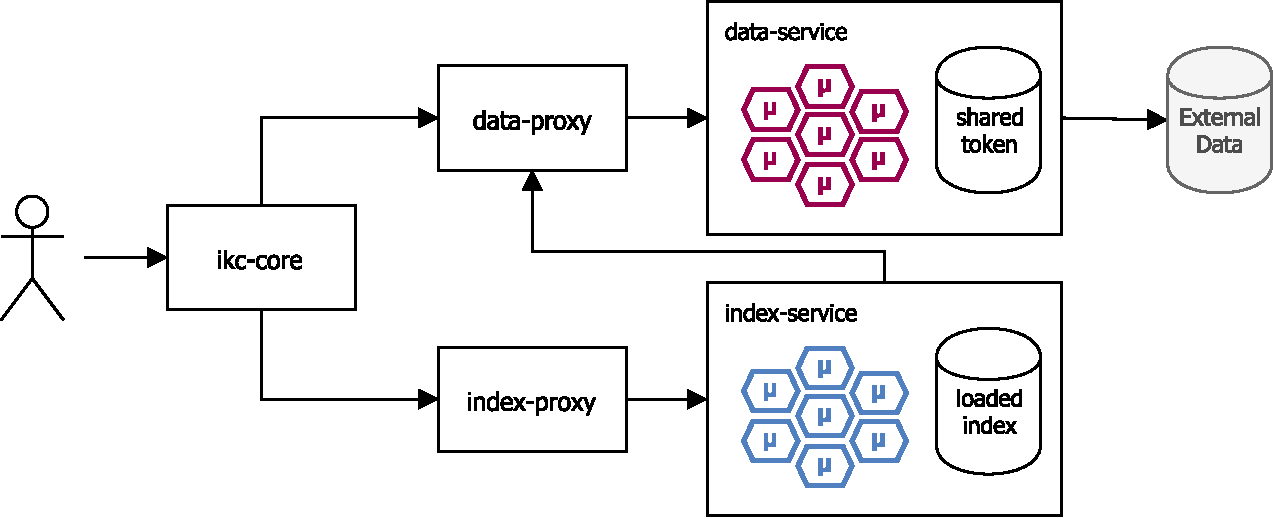
\includegraphics[width=1\textwidth]{Microservice}
    \caption{Überblick: MicroServices}
    \label{fig:micro-services}
    \end{figure}

